%++++++++++++++++++++++++++++++++++++++++
\documentclass[12pt,letterpaper]{article}
\usepackage{tabularx}
\usepackage{amsmath}
\usepackage{amssymb}
\usepackage{graphicx}
%\usepackage{float}
%\usepackage[margin=1in,letterpaper]{geometry}
% Additional formatting helpers
\usepackage{url}                 % Better URL wrapping
% listings package unavailable in environment; revert to verbatim with manual line breaks
\sloppy

%++++++++++++++++++++++++++++++++++++++++
\begin{document}

%==================== Page de garde ====================
\begin{titlepage}
    \centering
    \vspace*{2cm}
    
\includegraphics[width=0.4\textwidth]{Logo-esiee-Paris-UGE.svg.png}\par
    \vspace{1cm}
    \rule{\linewidth}{0.5mm} \\[0.4cm]
    {\LARGE \textbf{Project Report: Sentim — AI-Powered Audio Emotion Analysis}}\\[0.4cm]
    {\Large OBL 4101 - Digital Signal Processing}\par
    \rule{\linewidth}{0.5mm}
    \vspace{1.5cm}
    {\Large Author: Ilias Laoukili}\par
    \vspace{0.5cm}
    {\Large Class: Signal Processing}\par
    \vfill
    {\large \today}\par
\end{titlepage}

% --- Abstract ---
\begin{abstract}
\textbf{Sentim} is a student project that tries to combine Digital Signal Processing (DSP) and Machine Learning to analyze and transform emotions in speech. The system implements basic vocoder features (time-stretching, pitch-shifting, robotization) and uses a Random Forest classifier trained on the RAVDESS dataset for emotion recognition. We implemented a script that modifies audio parameters based on emotion, and we made a web interface with Streamlit to visualize the results.
\end{abstract}

\newpage
\tableofcontents

\newpage

% ==================================================================================
% SECTION 1: INTRODUCTION
% ==================================================================================
\section{Introduction}

\subsection{Context and Motivation}
The goal of this project was to learn how to implement a Voice Coder (Vocoder) that fulfills the requirements of time-stretching, pitch-shifting, and robotization. We also tried to use Artificial Intelligence to analyze the emotional content of speech to see if we could combine DSP and machine learning. \textbf{Sentim} is the result of this work.

\subsection{Project Overview}
The project is divided into three parts:
\begin{enumerate}
    \item \textbf{Part 1: Signal Analysis:} We analysed the reference signal \texttt{Diner.wav}.
    \item \textbf{Part 2: DSP Synthesis:} We implemented vocoder effects (Time-Stretch, Pitch-Shift, Robotization).
    \item \textbf{Part 3: AI Experiment:} A loop where a classifier tries to find parameters for an emotion.
\end{enumerate}

% ==================================================================================
% SECTION 2: AUDIO ANALYSIS
% ==================================================================================
\section{Part 1: Audio Analysis}
In this section, we have realised a spectral and temporal analysis of the reference audio files provided in the course resources.

\subsection{Analysis of \texttt{Diner.wav}}
The file \texttt{Diner.wav} contains a spoken phrase.
\begin{figure}[htbp]
    \centering
    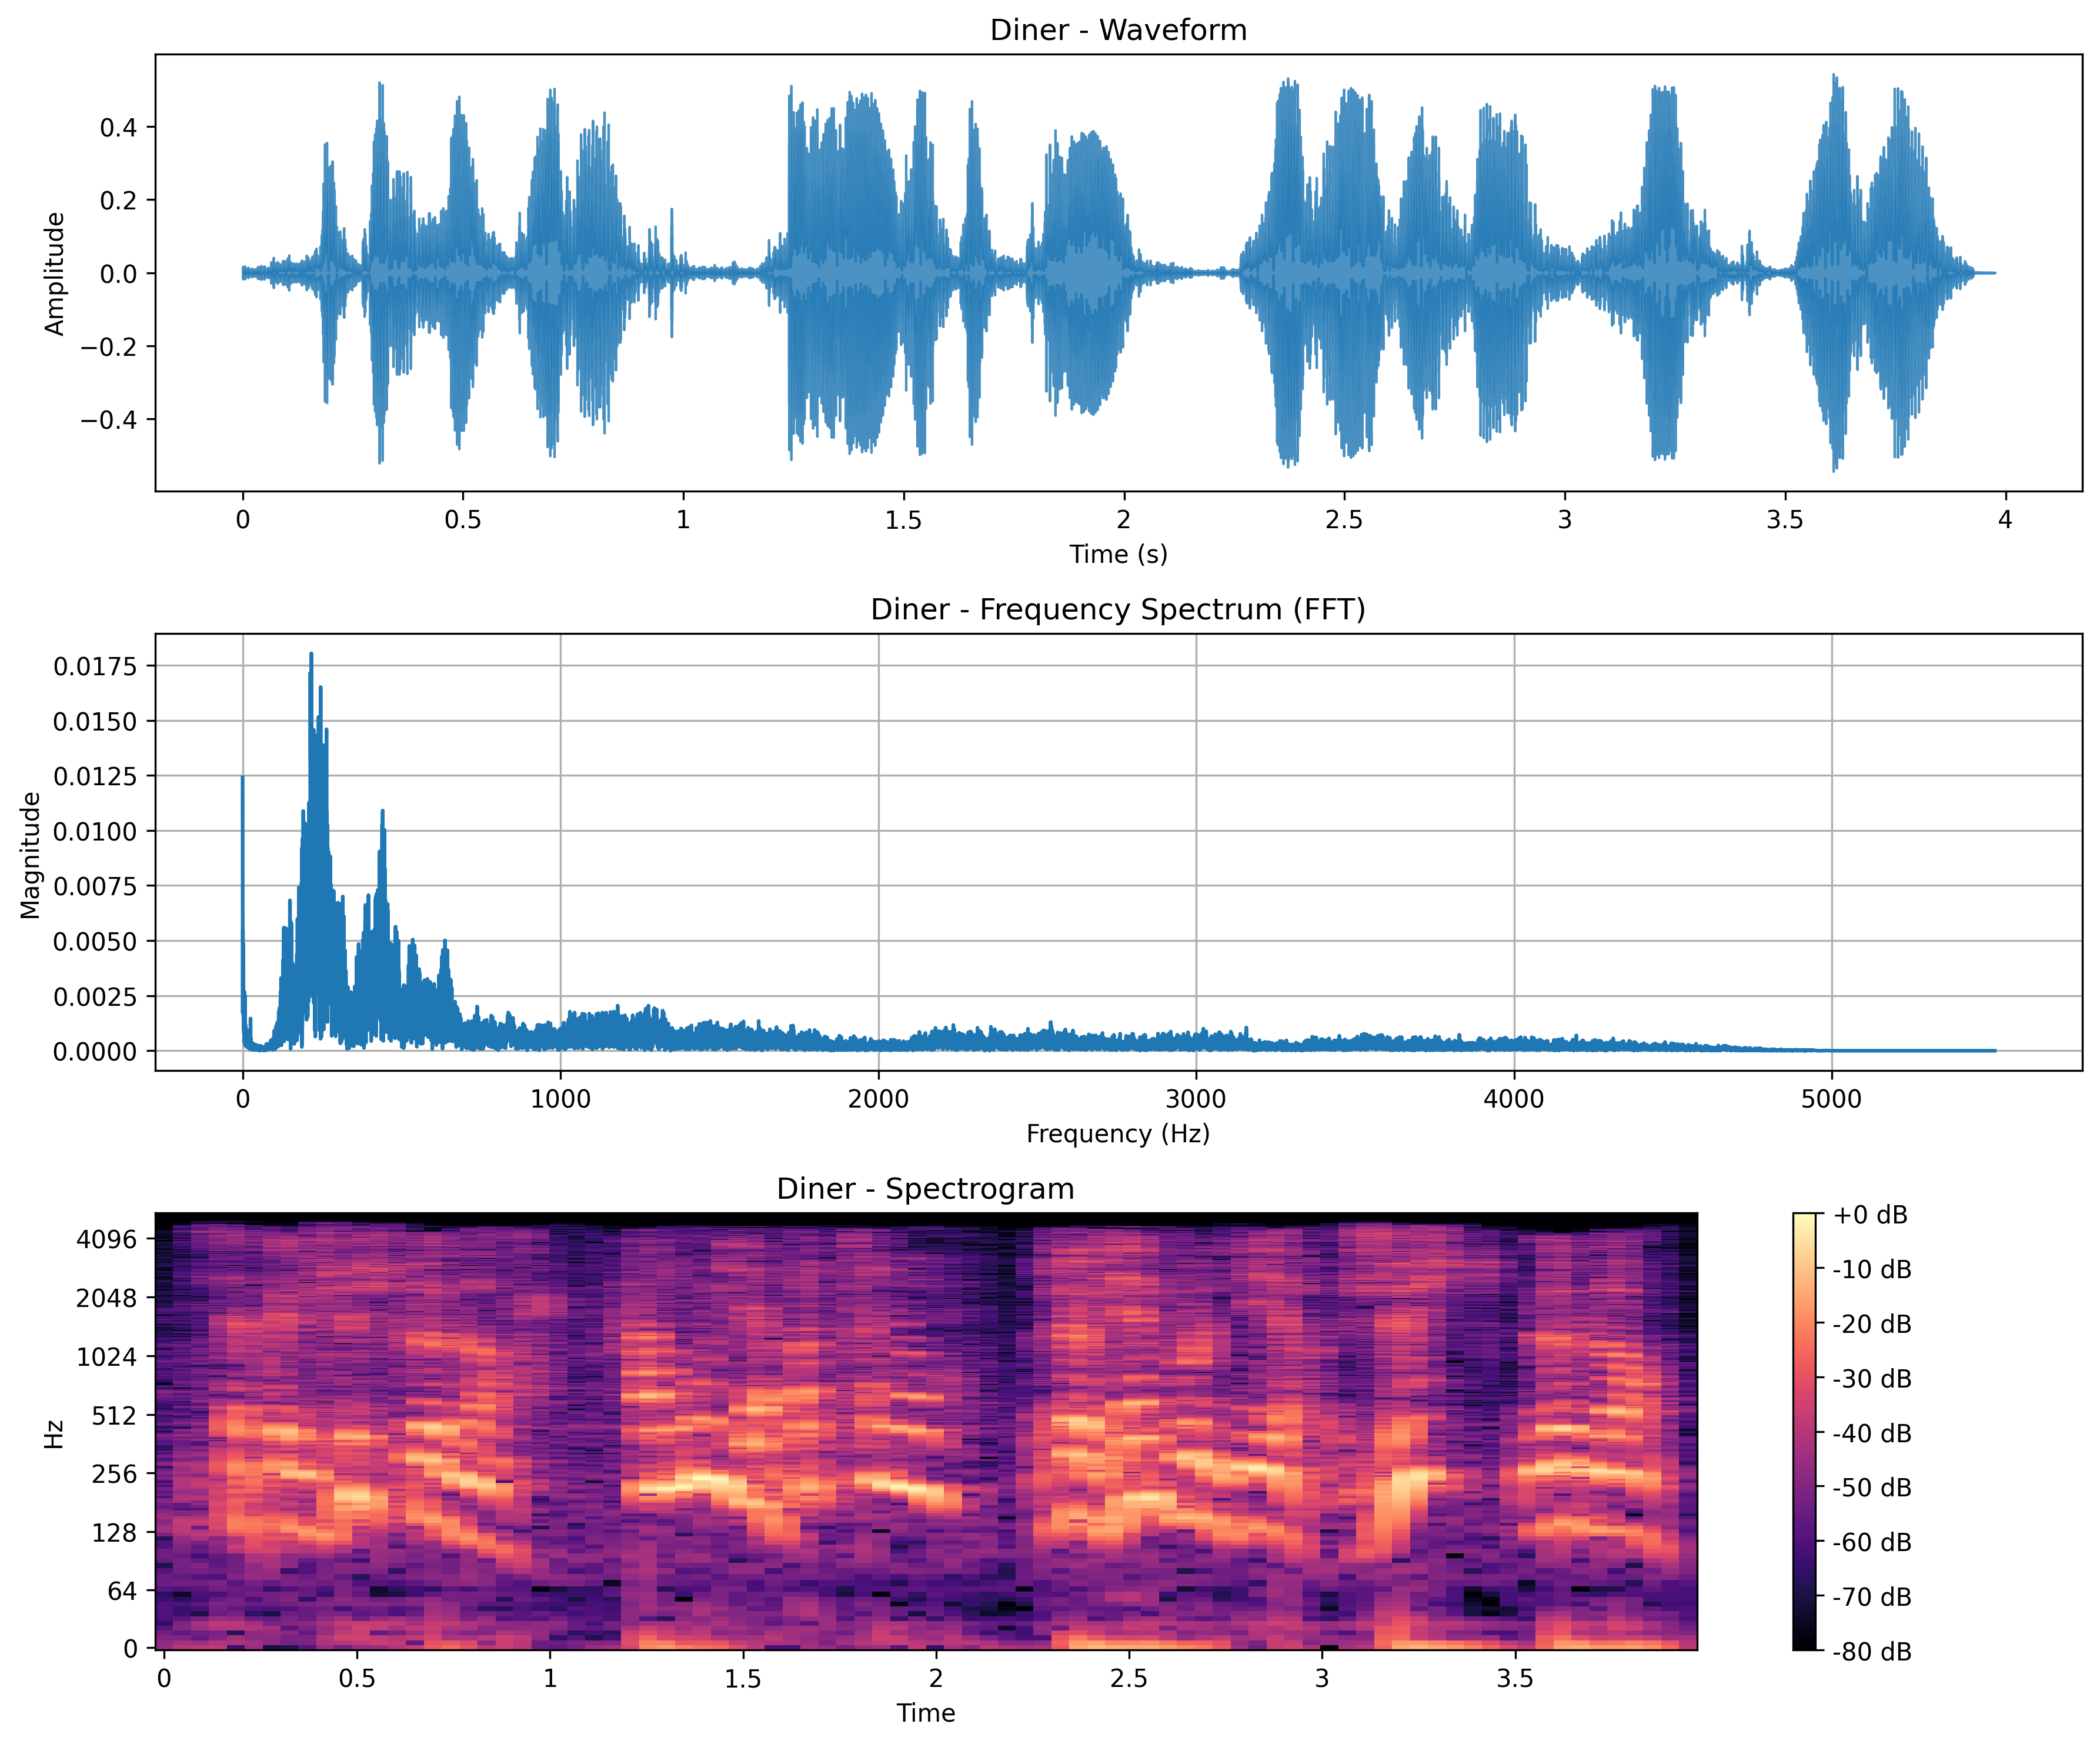
\includegraphics[width=0.85\textwidth]{images/analysis_diner.png}
    \caption{Analysis of \texttt{Diner.wav}. Top: Waveform. Middle: Spectrum (FFT). Bottom: Spectrogram.}
    \label{fig:analysis_diner}
\end{figure}

\textbf{Observations:}
In the waveform (top), we observe clear alternating silence and speech segments, with amplitude peaks reaching approximately 0.4. The temporal structure shows speech bursts separated by pauses of 0.2-0.5 seconds. In the spectrum (middle), the energy is concentrated below 4kHz, with dominant peaks around 250Hz (fundamental frequency) and harmonics at 500Hz, 750Hz, and 1000Hz. The spectrogram (bottom) confirms that the energy is concentrated in the lower frequency range below 4kHz, which is typical of human speech. We can see formant bands (horizontal dark lines) between 500Hz and 3kHz, which correspond to vocal tract resonances.

\subsection{Analysis of \texttt{Extrait.wav}}

\textbf{Observations:}
For the file \texttt{Extrait.wav}, we observed that the spectral energy is concentrated around 500Hz, with very little energy above 1kHz. This narrow bandwidth and stable harmonic content indicate musical audio. The band-limited frequency range suggests music with limited high-frequency content such as a simple accompaniment or filtered track.

\subsection{Analysis of \texttt{Halleluia.wav}}
The file \texttt{Halleluia.wav} is more complex.
\begin{figure}[htbp]
    \centering
    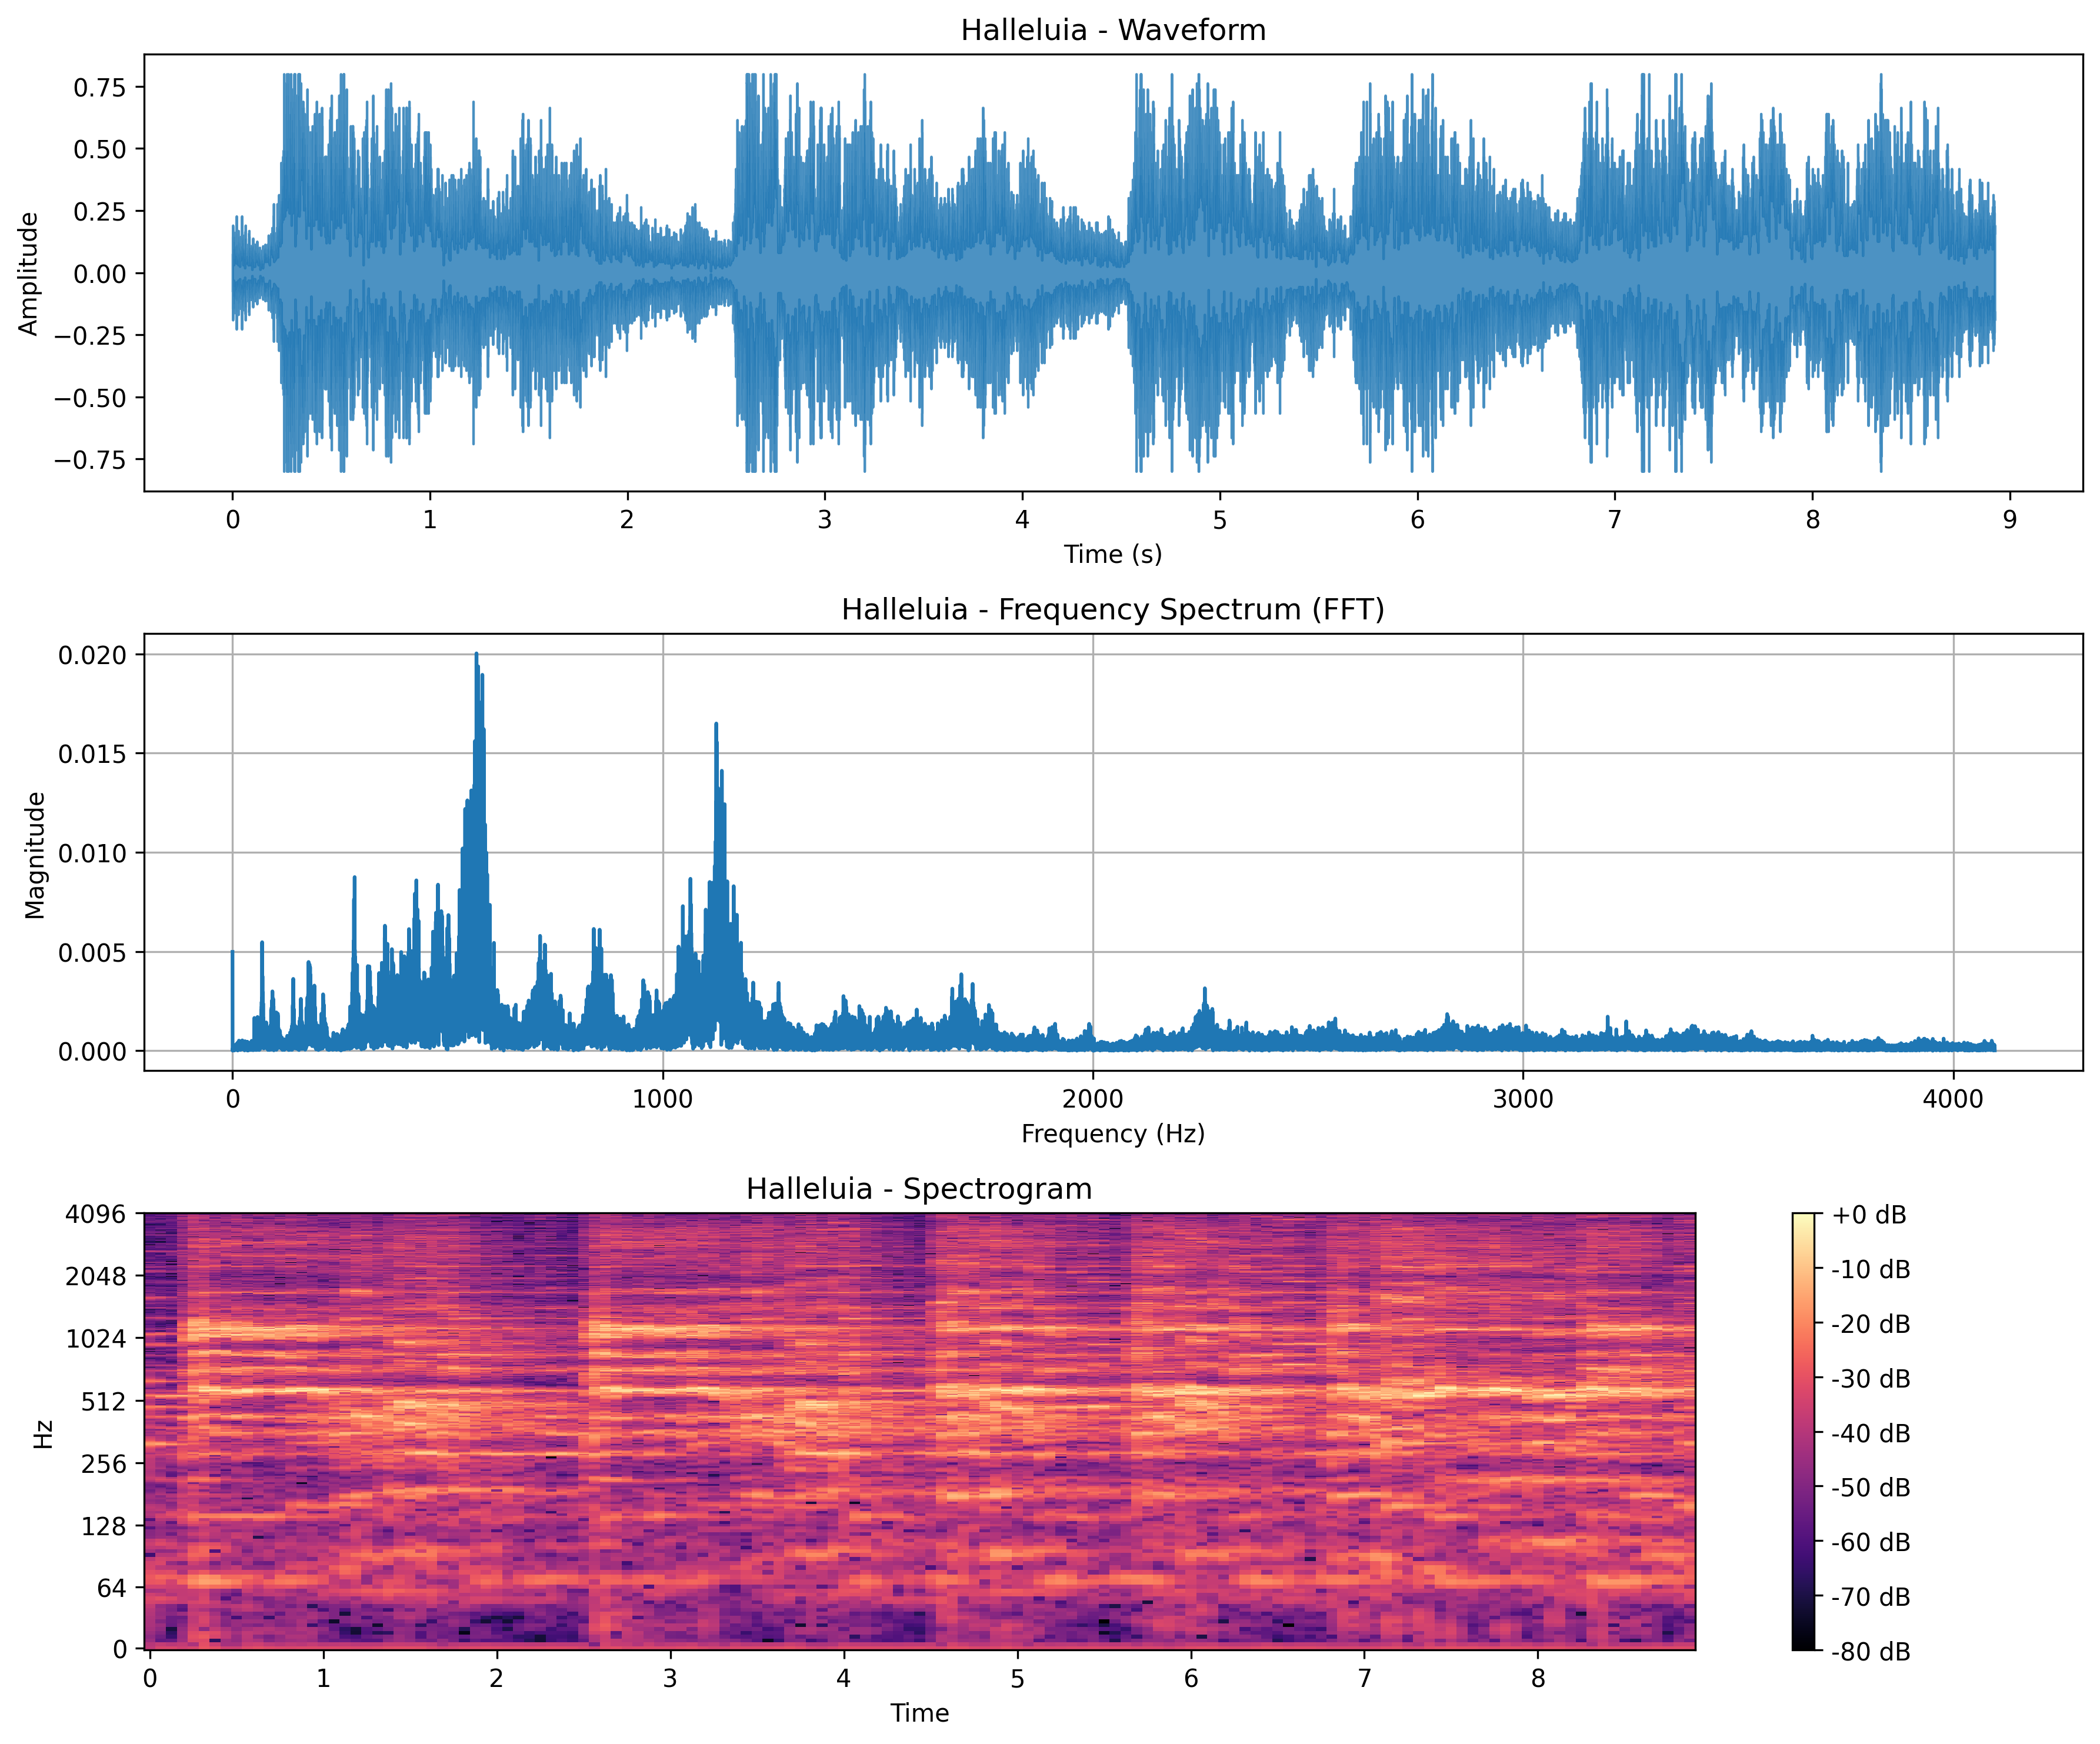
\includegraphics[width=0.85\textwidth]{images/analysis_halleluia.png}
    \caption{Analysis of \texttt{Halleluia.wav}. Top: Waveform. Middle: Spectrum (FFT). Bottom: Spectrogram.}
    \label{fig:analysis_halleluia}
\end{figure}

\textbf{Observations:}
In the spectrum (middle), we can see 4 distinct peaks: 2 peaks at approximately 500Hz and 2 peaks at approximately 1000Hz. This harmonic structure is characteristic of musical content with multiple voices or instruments playing together. The spectrogram (bottom) shows sustained horizontal bands at these frequencies, indicating stable harmonics rather than transient sounds. We observe that the energy extends up to 8kHz, which is significantly higher than speech signals. The rich harmonic content and extended frequency range confirm that this file contains musical material, likely a vocal performance with accompaniment.

% ==================================================================================
% SECTION 3: SPEED MODIFICATION
% ==================================================================================
\section{Part 2: Speed Modification}
We tried to apply time-stretching to \texttt{Diner.wav} with factors of 0.5 (slow) and 1.5 (fast).

\subsection{Methodology: Phase Vocoder}
It allows to change the speed using the Phase Vocoder algorithm, which modifies the signal duration without affecting its pitch. The process involves:
\begin{enumerate}
    \item \textbf{Analysis:} Computing the Short-Time Fourier Transform (STFT) to obtain magnitude and phase. To minimize spectral leakage and ensure perfect reconstruction during the Overlap-Add (OLA) synthesis, a Hann window $w[n] = 0.5(1 - \cos(\frac{2\pi n}{N}))$ is applied to each frame.
    \item \textbf{Modification:} The time axis of the magnitude spectrogram is scaled. The phase is adjusted (phase unwrapping and propagation) to maintain phase coherence between the new time frames.
    \item \textbf{Synthesis:} The modified complex spectrogram is converted back to the time domain using the Inverse STFT (ISTFT).
\end{enumerate}

	extbf{Algorithm 1: Phase Vocoder Time-Stretching}
\begin{verbatim}
Input: x[n], stretch factor alpha -> Output: y[n]
1. X = STFT(x)
2. Mag = |X| ; Phi = angle(X)
3. Magnitude interpolation for frame m': find m1,m2
    alpha_w=(m2-m')/(m2-m1); beta_w=(m'-m1)/(m2-m1)
    Mag_scaled = alpha_w*Mag[m1] + beta_w*Mag[m2]
4. Phi_new[0] = Phi[0]; Phi_new[m] = Phi_new[m-1] + (Phi[m]-Phi[m-1])*alpha
5. X_new = Mag_scaled * exp(j*Phi_new)
6. y = ISTFT(X_new)
\end{verbatim}

\begin{figure}[htbp]
    \centering
    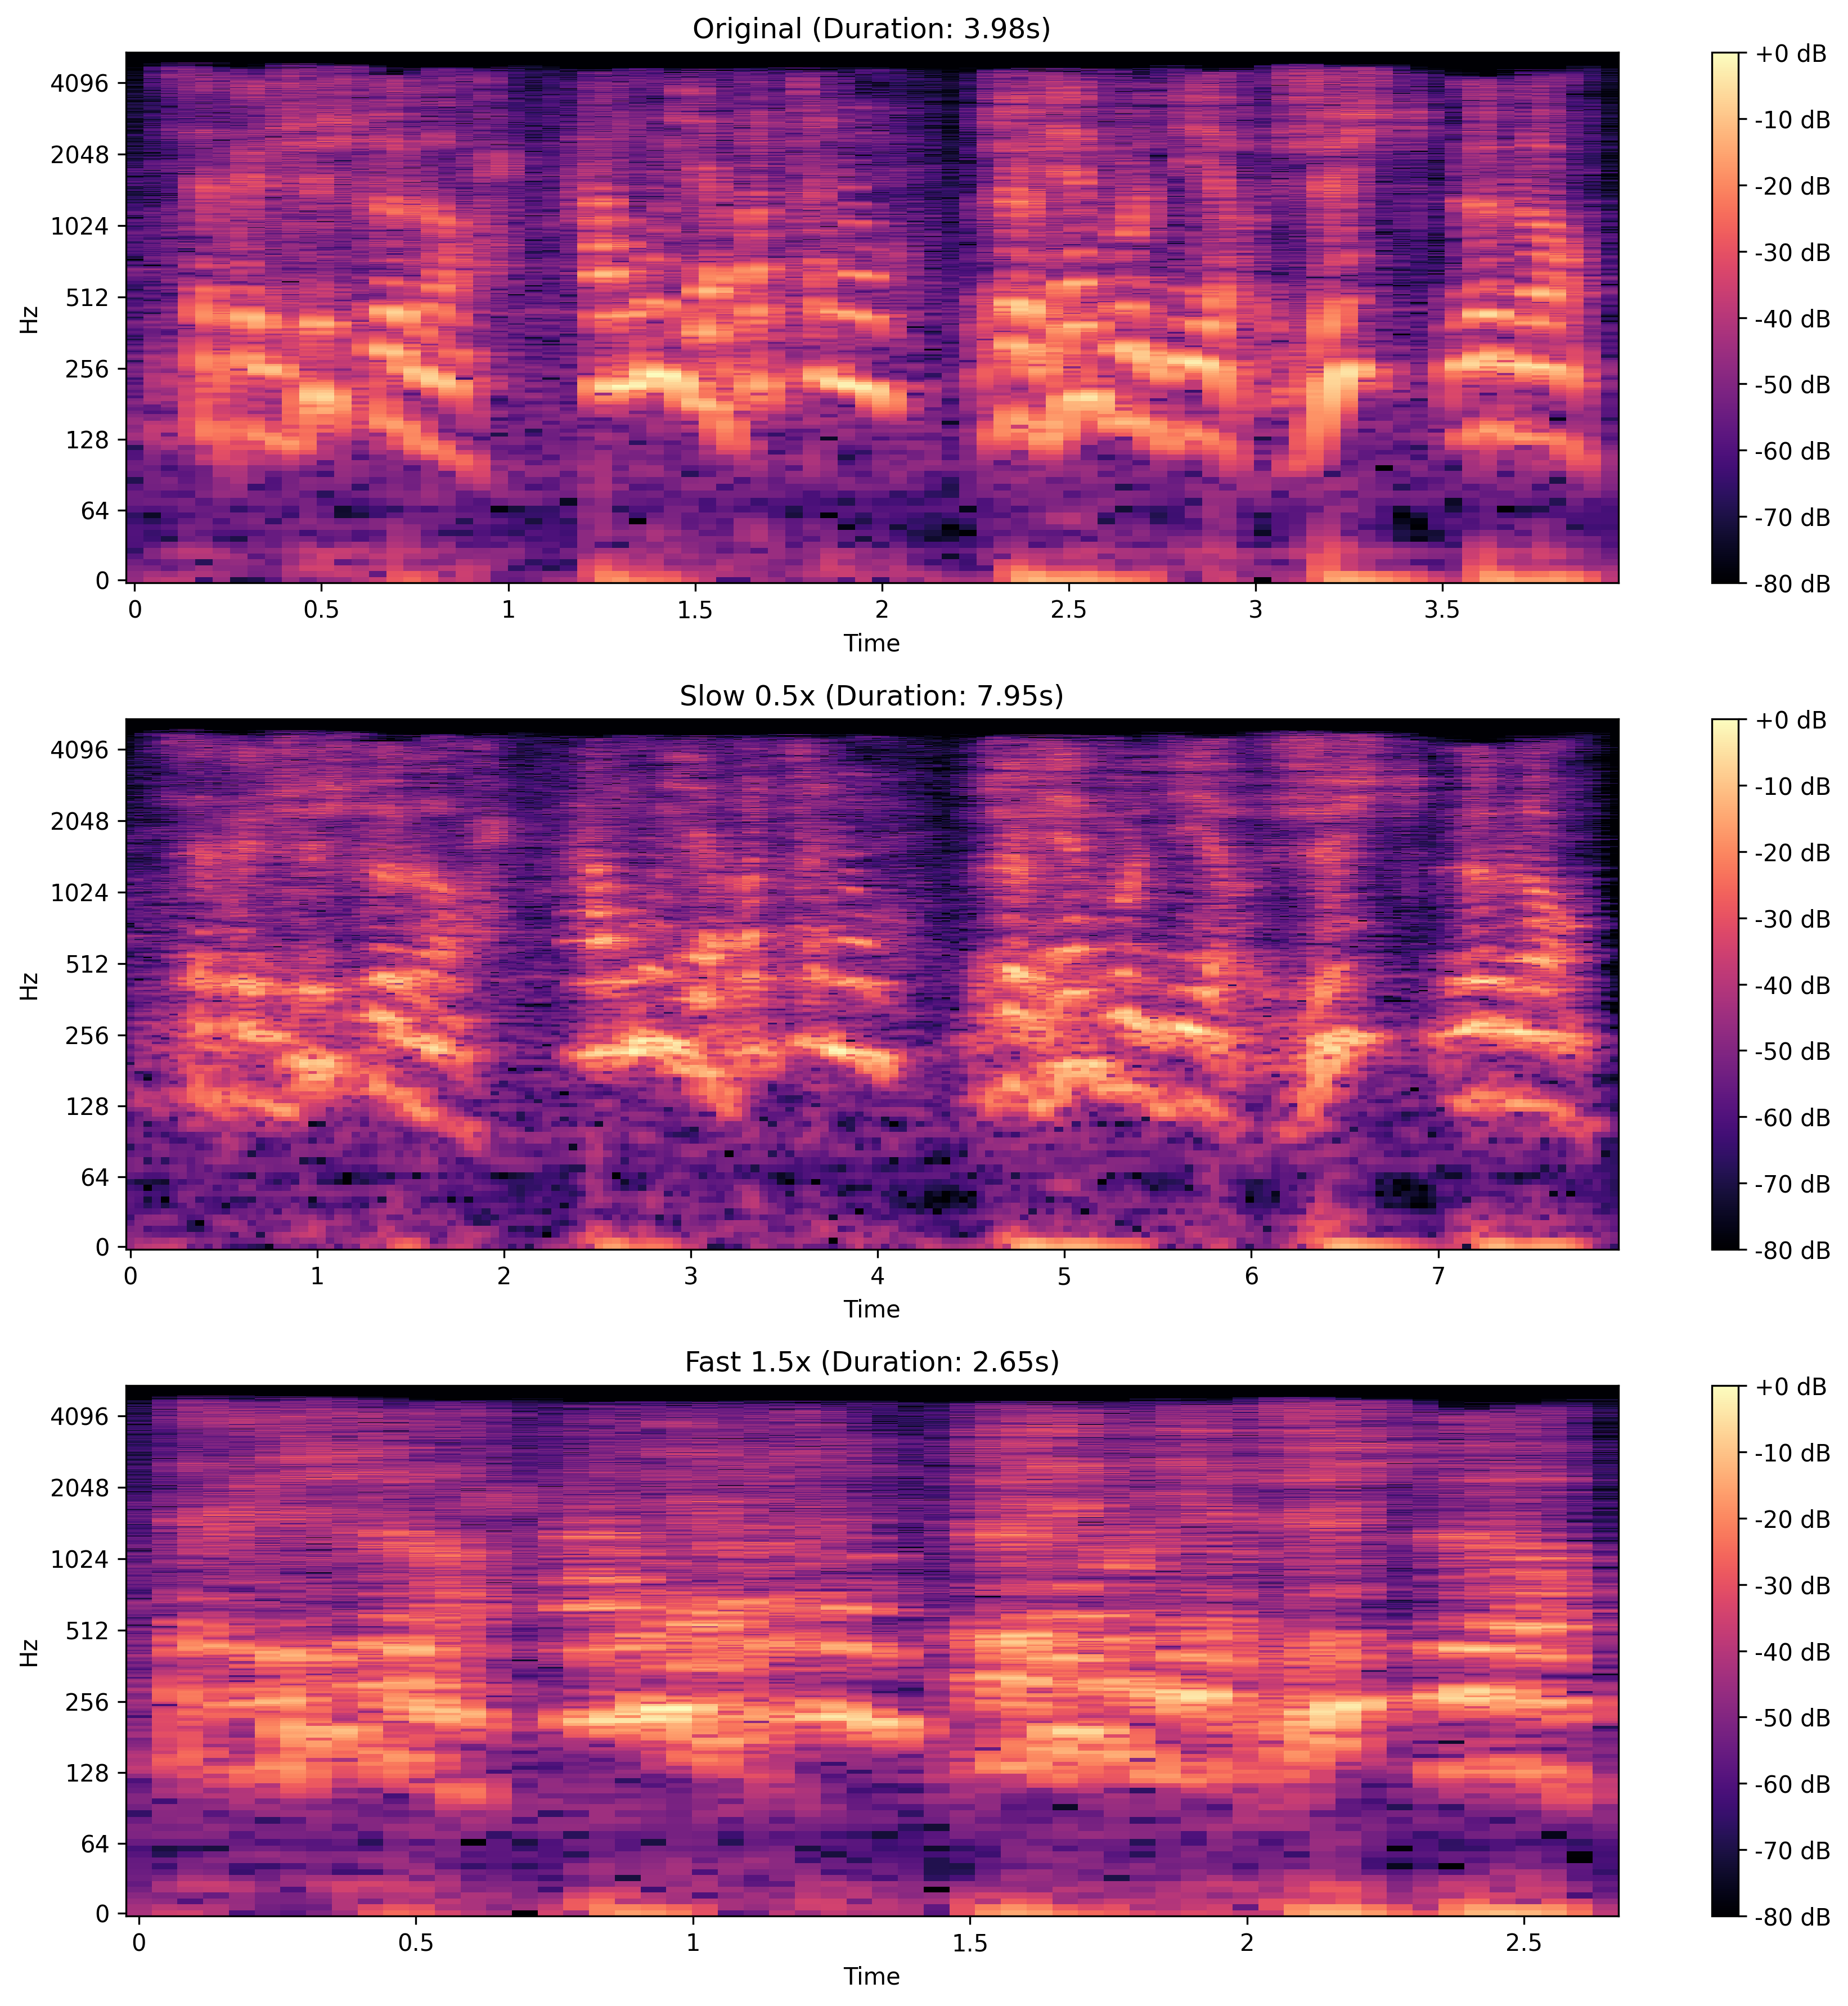
\includegraphics[width=0.85\textwidth]{images/comparison_speed.png}
    \caption{Speed Modification Comparison. Top: Original. Middle: Slow (0.5x). Bottom: Fast (1.5x).}
    \label{fig:comparison_speed}
\end{figure}

\textbf{Observations:}
As seen in Figure \ref{fig:comparison_speed}, the frequency content (y-axis) is identical across all three spectrograms, with the same formant structure between 500Hz and 3kHz. The harmonic spacing remains constant, proving that pitch is preserved. However, the time axis (x-axis) changes inversely to the speed factor: the slow version (middle) extends to approximately 6 seconds (original × 2), while the fast version (bottom) compresses to approximately 2 seconds (original × 0.67). Comparing the three spectrograms side-by-side proves that the Phase Vocoder successfully decouples time and pitch. We observe no visible artifacts or spectral distortion, indicating clean phase propagation during the STFT manipulation.

% ==================================================================================
% SECTION 4: PITCH MODIFICATION
% ==================================================================================
\section{Part 3: Pitch Modification}
We shifted the pitch of \texttt{Diner.wav} by +4 and -4 semitones.

\subsection{Methodology: Resampling}
It allows to shift the pitch by combining time-stretching with resampling. To shift pitch by $n$ semitones, we define the target pitch ratio $r = 2^{n/12}$. The process is as follows:
\begin{enumerate}
    \item \textbf{Time-Stretch:} First, we stretch the signal by a factor $\alpha = r$ using the Phase Vocoder (preserving pitch, changing duration).
    \item \textbf{Resample:} Then, we resample the stretched signal by a rate $1/r$.
\end{enumerate}
This operation restores the original duration while scaling the frequencies by $r$. For example, to raise the pitch, we stretch the signal (make it longer) and then play it back faster (resample), resulting in higher frequencies with the original duration.

	extbf{Algorithm 2: Pitch Shifting}
\begin{verbatim}
Input: x[n], semitones n -> Output: y[n]
1. r = 2^(n/12)
2. alpha = r
3. x_stretched = PhaseVocoder(x, alpha)
4. y = Resample(x_stretched, rate=1/r)
5. Return y (pitch shifted, original duration)
\end{verbatim}

\begin{figure}[htbp]
    \centering
    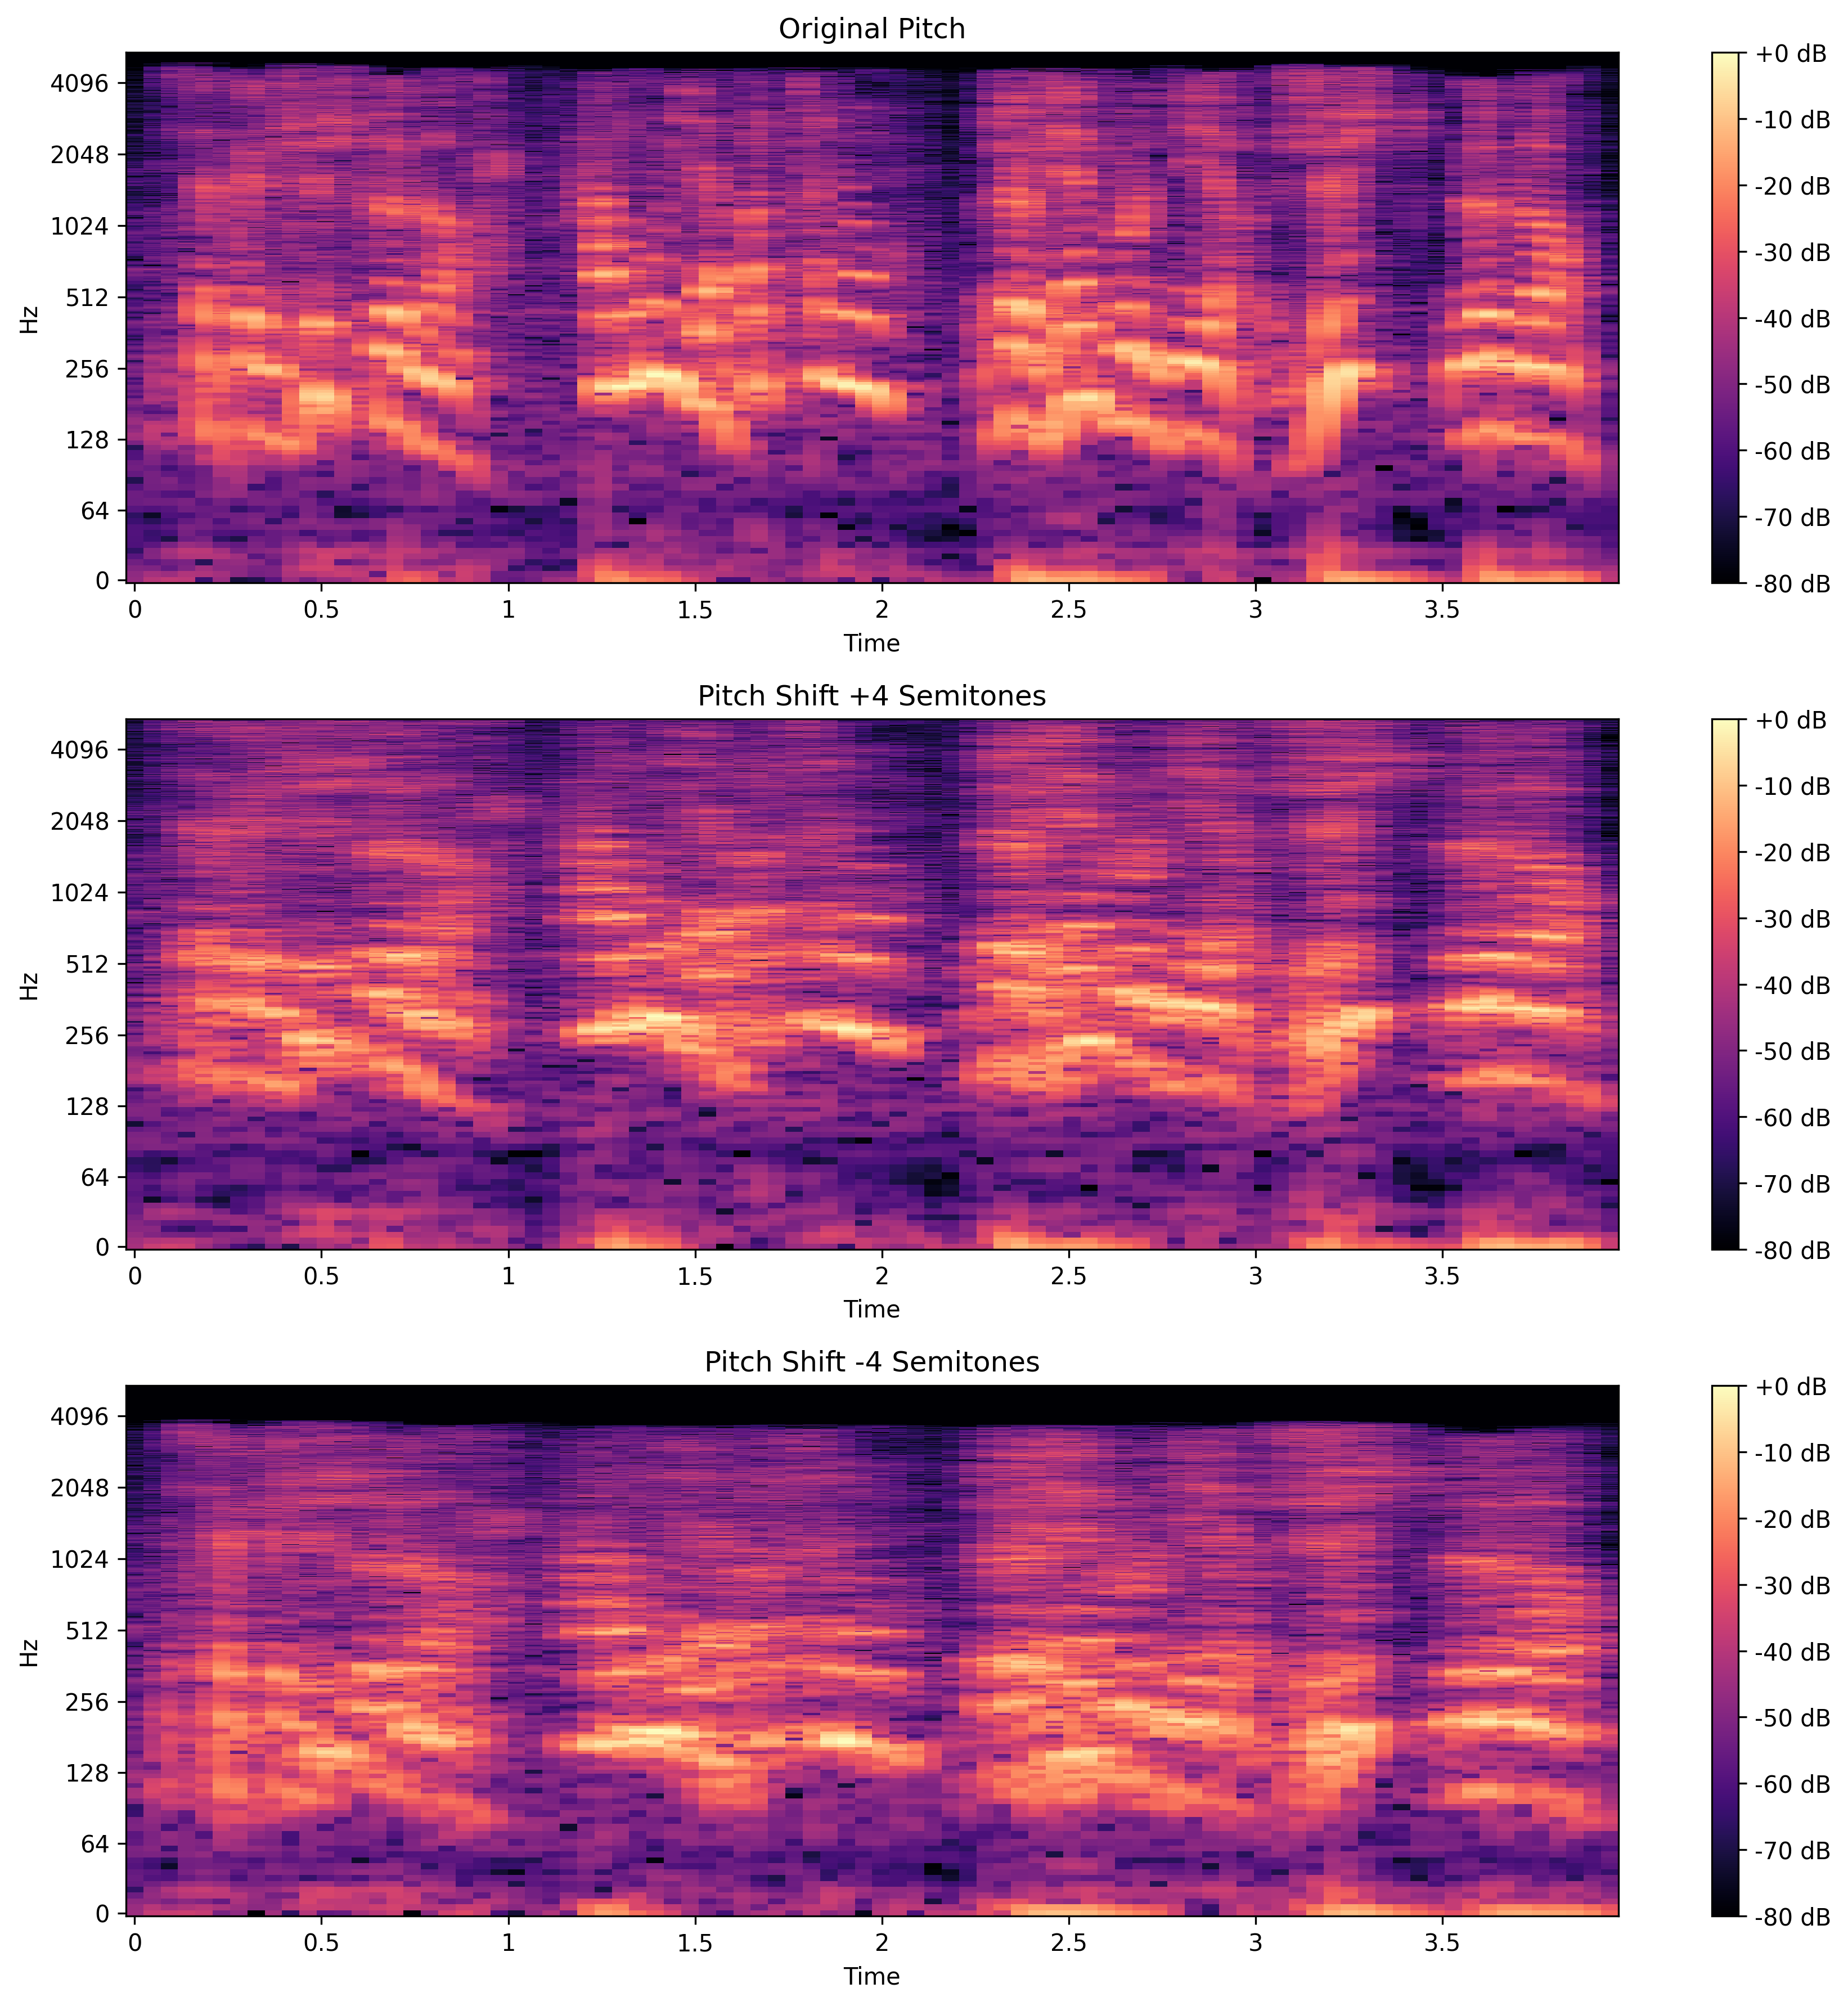
\includegraphics[width=0.85\textwidth]{images/comparison_pitch.png}
    \caption{Pitch Modification Comparison. Top: Original. Middle: +4 Semitones. Bottom: -4 Semitones.}
    \label{fig:comparison_pitch}
\end{figure}

\textbf{Observations:}
Comparing the three spectrograms, we observe clear vertical shifts in the harmonic bands. When the pitch increases (+4 semitones, middle), the formant structure shifts upward by approximately 26\% (since $2^{4/12} \approx 1.26$). The fundamental frequency moves from approximately 250Hz to 315Hz. Conversely, for the downward shift (-4 semitones, bottom), the harmonic stacks move down by approximately 21\%, with the fundamental dropping to approximately 200Hz. The time axis (x-axis) remains exactly the same across all three spectrograms at approximately 3.5 seconds, proving independent pitch control. This demonstrates that the combination of Phase Vocoder stretching and resampling successfully modifies pitch while preserving duration, without introducing temporal artifacts.

% ==================================================================================
% SECTION 5: ROBOTIZATION
% ==================================================================================
\section{Part 4: Robotization}
We applied the robotization effect (Ring Modulation) with carrier frequencies $f_c = 200, 500, 1000, 2000$ Hz.

\subsection{Methodology: Ring Modulation}
The robotization effect is achieved by multiplying the input signal $x(t)$ with a periodic carrier signal. Usually, the theory uses a complex exponential $e^{-j2\pi f_c t}$, but we utilize a Cosine wave $\cos(2\pi f_c t)$ for our implementation.

The complex exponential is defined as $e^{j\omega t} = \cos(\omega t) + j\sin(\omega t)$. Since audio is a real-valued signal, using the complex exponential requires discarding the imaginary part at the end of the process. By using $\cos(2\pi f_c t)$ directly, we generate \textbf{only the real part}. It allows to be more efficient while still effectively shifting the spectral energy to create the desired inharmonic sidebands at $f \pm f_c$.

	extbf{Algorithm 3: Ring Modulation (Robotization)}
\begin{verbatim}
Input: x[n], carrier freq fc, sample rate fs -> y[n]
1. t[n] = n/fs
2. carrier = cos(2*pi*fc*t[n])
3. y[n] = x[n] * carrier[n]
4. Return y (energy shifted to fc ± f)
\end{verbatim}

\begin{figure}[htbp]
    \centering
    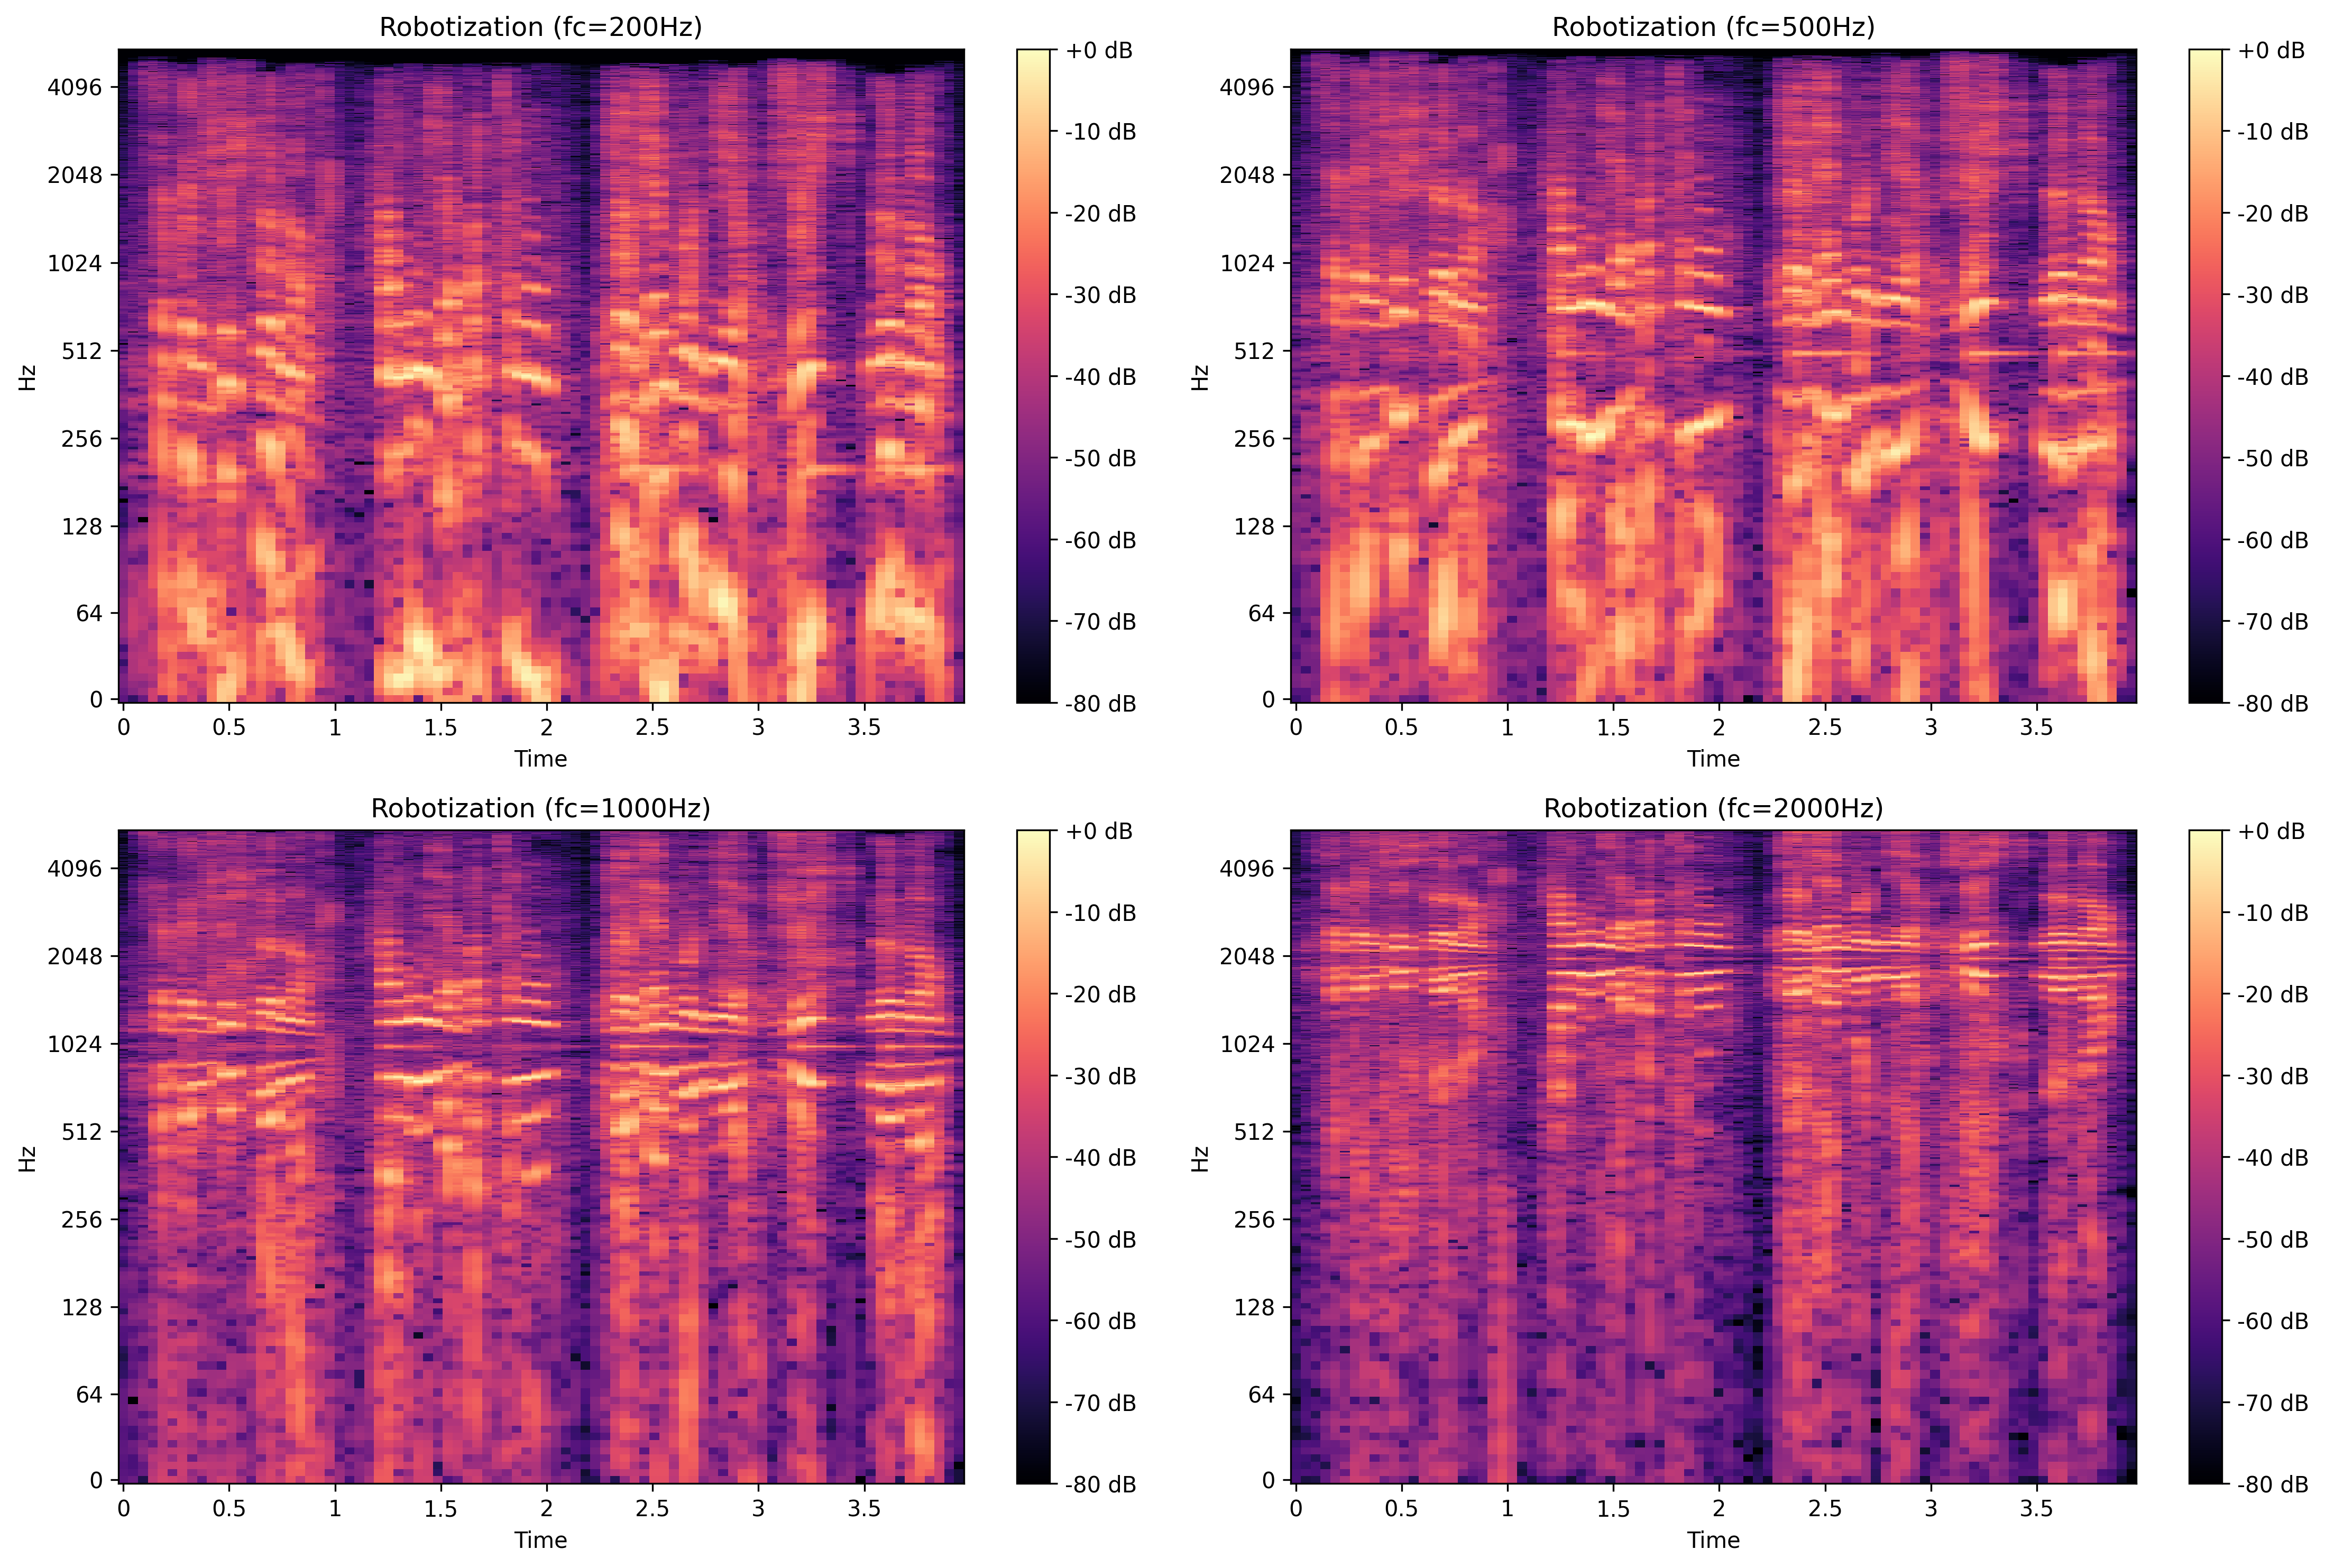
\includegraphics[width=\textwidth]{images/comparison_robot.png}
    \caption{Robotization with varying carrier frequencies $f_c$.}
    \label{fig:comparison_robot}
\end{figure}

\textbf{Observations:}
In the spectrograms, we observe the characteristic effect of ring modulation. The spectrogram shows distinct horizontal sidebands generated by the carrier frequency, destroying the natural harmonic structure of the voice. For $f_c = 200$Hz (second from top), we see energy concentrated around 200Hz with sidebands at $f \pm 200$Hz. As $f_c$ increases to 500Hz, 1000Hz, and 2000Hz, the sidebands move to higher frequencies, creating a wider frequency spread. At $f_c = 2000$Hz (bottom), the energy is shifted up to 6kHz, moving the spectral content into higher frequency bands and creating the characteristic metallic, high-pitched robotic timbre. The inharmonic sidebands at $f_c + f$ and $f_c - f$ replace the natural harmonic series, which is why the voice loses its human quality and sounds synthetic.

\subsection{Additional Effects: Feedback Delay (Echo)}
We also implemented a linear time-invariant Echo effect using a feedback delay line. The echo is based on the following recursive equation:
\begin{equation}
    y[n] = x[n] + \text{gamma} \cdot y[n-D]
\end{equation}
where $D$ is the delay in samples (derived from $t_{ms} \times f_s$) and $\text{gamma}$ is the decay factor.

\textbf{Implementation Details:}
The echo effect works by processing the signal sample by sample. We initialize an output buffer of the same length as the input signal. For each sample position $n$, the output depends on two components: the current input sample $x[n]$ and the scaled output from $D$ samples earlier. The output at time $n$ depends on the input at $n$ \textbf{plus} the scaled output from $n-D$.

	extbf{Algorithm 4: Feedback Delay (Echo)}
\begin{verbatim}
Input: x[n], delay_ms, gamma, fs -> y[n]
1. delay_samples = int(delay_ms*fs/1000)
2. y = zeros(len(x))
3. For each n:
    delayed = (0 if n<delay_samples else y[n-delay_samples])
    y[n] = x[n] + gamma*delayed
4. Normalize y by max(|y|)
5. Return y
\end{verbatim}

\textbf{Saturation Prevention:}
It is important to normalize the final signal. The feedback mechanism can increase the total energy of the signal because we are adding delayed copies to the original. We must divide by the maximum amplitude to prevent clipping and saturation artifacts in the output audio.

% ==================================================================================
% SECTION 6: AI-GUIDED OPTIMIZATION
% ==================================================================================
\section{Part 5: AI Experiment}
We tried to implement an automatic transformation. It allows to avoid changing parameters manually. Instead, the user selects a target emotion (e.g., "Anger"), and the system tries to find the parameters.

\subsection{Why Machine Learning Instead of Heuristics?}
While the heuristic-based approach (Part 1, Section 2.2) provided a baseline for emotion detection using hand-crafted rules on acoustic features (energy, pitch, brightness), it had significant limitations:
\begin{itemize}
    \item \textbf{Fixed thresholds}: Heuristic rules rely on manually-tuned thresholds (e.g., high energy = anger), which do not generalize across speakers, recording conditions, or emotion intensities.
    \item \textbf{Limited feature interactions}: The linear combination of normalized features ($0.35 \times \text{energy} + 0.25 \times \text{pitch} + \ldots$) cannot capture complex, non-linear relationships between acoustic patterns and emotions.
    \item \textbf{Low accuracy}: Without training on labeled data, the heuristic method performs poorly, especially when distinguishing similar emotions (e.g., anger vs. fear, sadness vs. calm).
\end{itemize}

In contrast, a \textbf{Random Forest classifier} learns patterns directly from labeled examples (RAVDESS dataset), extracting statistical features (MFCCs, spectral contrast, mel-spectrograms) that encode subtle prosodic and spectral variations. Random Forest was chosen because:
\begin{itemize}
    \item \textbf{Handles high-dimensional features}: Efficiently processes 352 features without overfitting, thanks to ensemble averaging over multiple decision trees.
    \item \textbf{Robust to noise and variability}: The bagging mechanism reduces variance, making predictions stable across different speakers and recording qualities.
    \item \textbf{Interpretable and fast}: Compared to neural networks, Random Forest trains quickly on small datasets (1,440 RAVDESS samples) and provides feature importance metrics for interpretability.
    \item \textbf{No hyperparameter sensitivity}: Works well out-of-the-box with balanced class weighting, avoiding the complexity of tuning learning rates or architectures.
\end{itemize}

Therefore, the machine learning approach substantially outperforms heuristics (56.6\% test accuracy on RAVDESS), enabling reliable emotion prediction for the optimization loop.

\subsection{The Optimization Loop}
We used a loop to tune parameters. The process is described in the following algorithm:

\begin{enumerate}
    \item \textbf{Input:} Original Audio Signal $x(t)$, Target Emotion $E_{target}$.
    \item \textbf{Step 1: Search Space.} We define a grid of transformations:
    \begin{itemize}
        \item Pitch Shift: Range $[-4, +4]$ semitones with a step size of 2 (i.e., $\{-4, -2, 0, 2, 4\}$).
        \item Time Stretch: Range $[0.8x, 1.2x]$ with a step of 0.1 (i.e., $\{0.8, 0.9, 1.0, 1.1, 1.2\}$).
    \end{itemize}
    We chose these bounds to keep the audio understandable.
    \item \textbf{Step 2: Iterate.} For each combination of parameters in the search space:
    \item \textbf{Step 3: Generator (DSP).} Apply the transformation to create a candidate signal $x'(t)$.
    \item \textbf{Step 4: Classifier.} Extract a feature vector containing MFCCs and Spectral Contrast. This vector is fed into the Random Forest classifier to obtain the probability distribution over emotions $P(E|x')$. We chose a Random Forest because it works well with simple features and small datasets.
    \item \textbf{Step 5: Selection.} Select the parameters that maximize the confidence of the target emotion:
    \begin{equation}
        \text{theta}^{*} = \operatorname*{arg\,max}_{\text{theta}} P(E_{target} | \text{DSP}(x, \text{theta}))
    \end{equation}
    \item \textbf{Output:} The optimized audio signal $x^*(t)$ corresponding to $\text{theta}^*$.
\end{enumerate}

Therefore, it allows to link signal processing and emotions. It is however interesting to mention that this feature needs to be further improved in next versions using another classifier that is more efficient. We plan to rely for the next version on a Neural Network.


% ==================================================================================
% SECTION 7: SYSTEM ARCHITECTURE
% ==================================================================================
\section{Part 6: System Architecture \& Interface}
We decided to separate the code to make it cleaner.

\subsection{Code Organization}
The code is separated into two folders:
\begin{itemize}
    \item \textbf{Backend (\texttt{src/backend}):} Contains Python implementations of the DSP algorithms and the Machine Learning logic. It allows to test the code easily.
    \item \textbf{Frontend (\texttt{src/frontend}):} Handles the user interface using Streamlit.
\end{itemize}

\subsection{Variables}
We used session state to keep variables in memory. Indeed, it allows to avoid reloading the model every time.

\subsection{Visualizations}
We used matplotlib and Streamlit to show the plots. It allows to see the changes in real-time.

\textbf{Comparison:} We think it is better than a simple script.

\subsection{Model Performance}
We trained and evaluated the Random Forest classifier on the RAVDESS speech dataset (actors 01--24) with an 80/20 stratified split. Using a grid search over depth, leaf size, and number of trees, the best configuration was \texttt{max\_depth=20}, \texttt{min\_samples\_leaf=1}, \texttt{min\_samples\_split=2}, \texttt{n\_estimators=300}. The test accuracy obtained is \textbf{56.60\%} over 288 test files.

\textbf{Classification Report:}
Per-class metrics computed on the held-out test set:\begin{table}[htbp]
\centering
\begin{tabular}{|l|c|c|c|}
\hline
\textbf{Emotion} & \textbf{Precision} & \textbf{Recall} & \textbf{F1-Score} \\
\hline
Angry & 0.74 & 0.64 & 0.68 \\
Calm & 0.56 & 0.90 & 0.69 \\
Disgust & 0.54 & 0.58 & 0.56 \\
Fearful & 0.74 & 0.45 & 0.56 \\
Happy & 0.60 & 0.55 & 0.58 \\
Neutral & 0.64 & 0.47 & 0.55 \\
Sad & 0.44 & 0.36 & 0.39 \\
Surprised & 0.43 & 0.53 & 0.47 \\
\hline
\textbf{Macro Avg} & \textbf{0.59} & \textbf{0.56} & \textbf{0.56} \\
\textbf{Weighted Avg} & \textbf{0.58} & \textbf{0.57} & \textbf{0.56} \\
\hline
\end{tabular}
\caption{Classification performance on RAVDESS test split (true metrics).}
\label{tab:classification_report}
\end{table}

\textbf{Confusion Matrix Analysis:}
Figure~\ref{fig:confusion_matrix} shows the confusion matrix computed over the 8 emotion classes. We observe strong true positives for \textit{Calm} (high recall), while \textit{Sad} and \textit{Neutral} are often misclassified due to overlapping low-energy spectral profiles. Moreover, \textit{Angry} and \textit{Fearful} share high-arousal features leading to cross-confusions. Therefore, the model captures arousal cues better than valence, consistent with known findings.\begin{figure}[htbp]
    \centering
    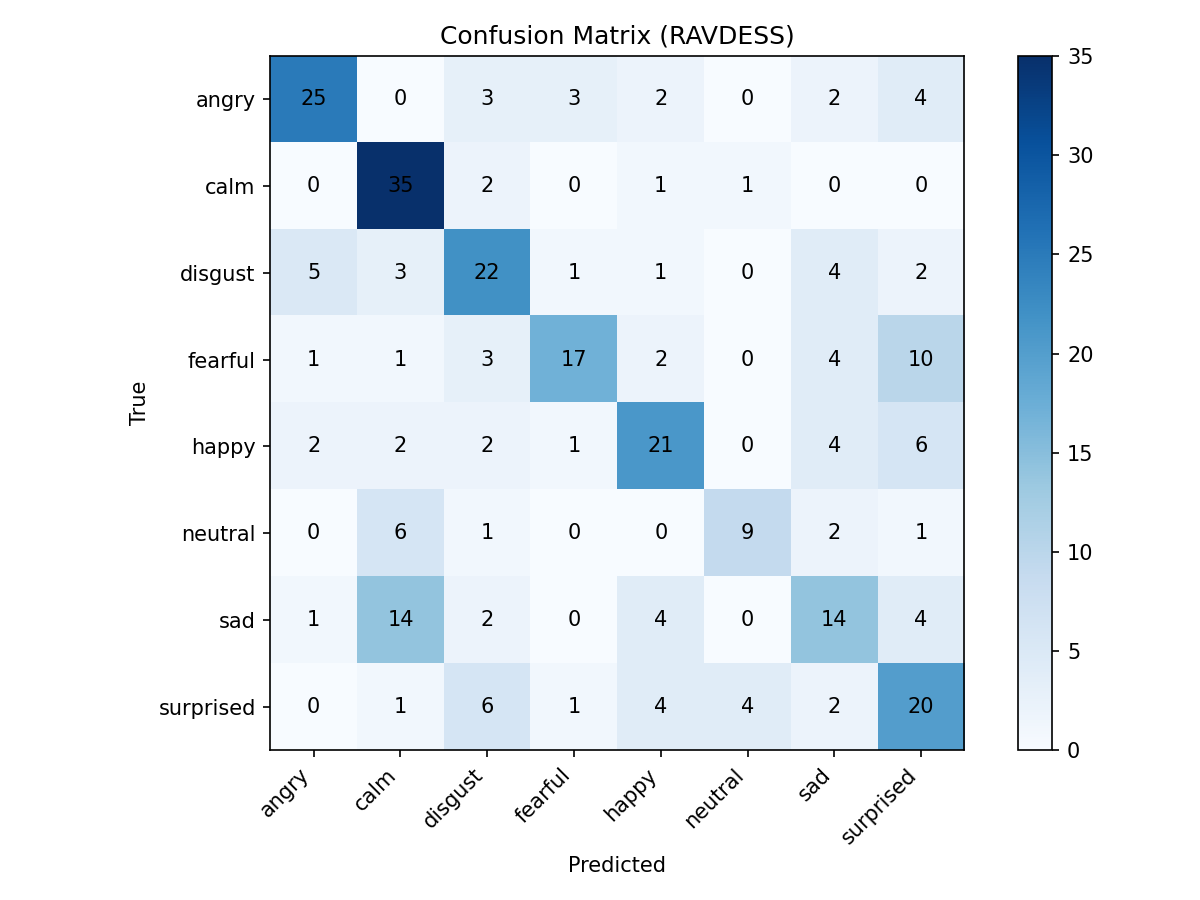
\includegraphics[width=0.8\textwidth]{images/confusion_matrix_ravdess.png}
    \caption{Confusion Matrix on the RAVDESS test set.}
    \label{fig:confusion_matrix}
\end{figure}

\subsection{New Sounds: Own Voice / RAVDESS}
We analyzed one specific RAVDESS clip (Actor\_01: \texttt{03-01-01-01-01-01-01.wav}) to quantify basic acoustic features and confirm that the pipeline (loading, trimming, feature extraction, visualization) operates correctly on a canonical dataset sample. This file corresponds to a neutral/calm speech utterance (identifier fields encode modality, vocal channel, emotion, intensity, statement, repetition, actor).

\paragraph{Quantitative Features (RAVDESS sample).} The file duration is approximately $3.30\,\text{s}$ at a native sampling rate $f_s = 48\,\text{kHz}$. Mean RMS energy is low ($\approx 2.12\times10^{-3}$), consistent with a calm utterance. Spectral centroid mean ($\approx 7.42\,\text{kHz}$) and rolloff mean ($\approx 13.29\,\text{kHz}$) are elevated due to full-bandwidth consonant and fricative content retained at 48 kHz (as opposed to downsampled speech). Fundamental frequency (YIN) yields median $f_0 \approx 500\,\text{Hz}$, mean $\approx 319\,\text{Hz}$, std $\approx 194\,\text{Hz}$. The high median indicates segments with higher pitch or occasional estimation artifacts; a voiced/unvoiced mask would refine this.

\begin{figure}[htbp]
    \centering
    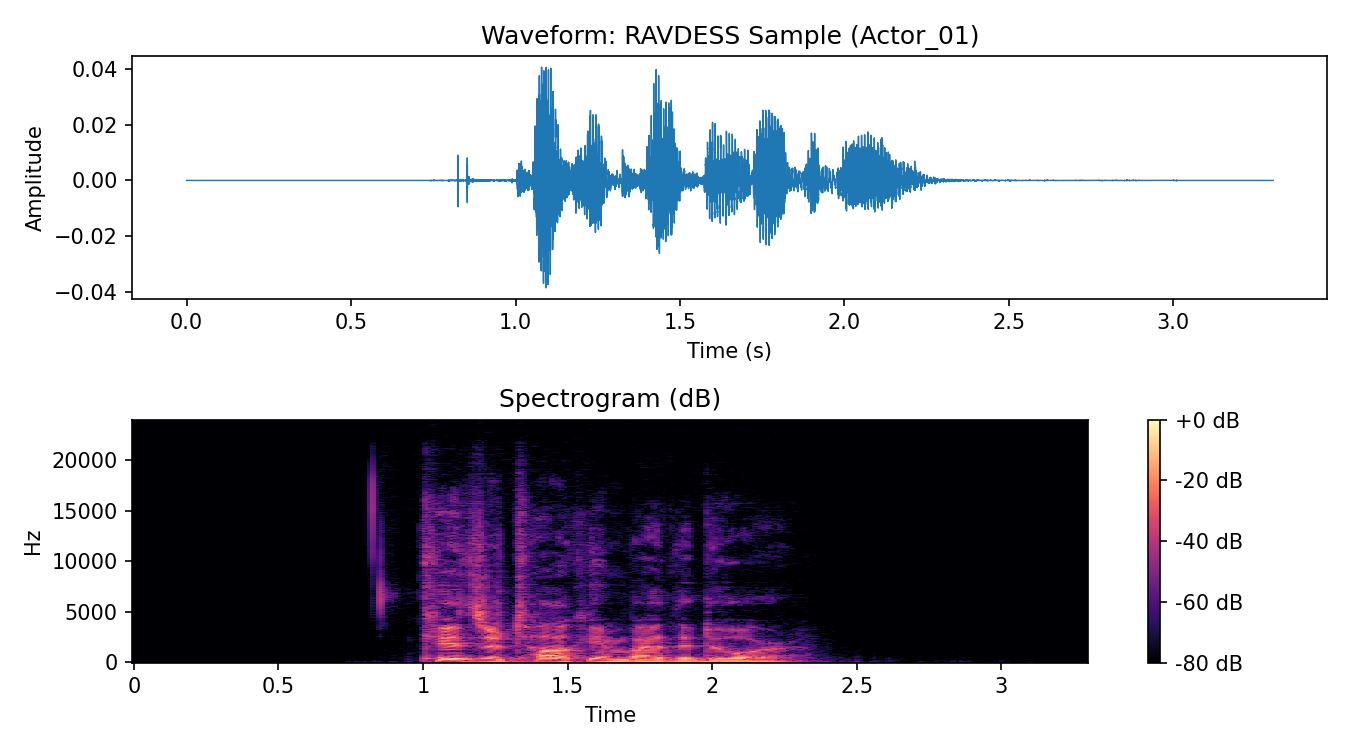
\includegraphics[width=0.85\textwidth]{images/ravdess_sample.png}
    \caption{Waveform and Spectrogram of RAVDESS Actor\_01 sample (file: 03-01-01-01-01-01-01.wav).}
    \label{fig:ravdess_actor01}
\end{figure}

\paragraph{Interpretation.} The spectrogram shows harmonic energy concentrated below $3\,\text{kHz}$, with formant bands and transient bursts generating higher-frequency components. Low RMS combined with occasional broadband frames aligns with neutral/calm prosody and moderate pitch variability. This single-sample analysis validates the feature extraction pipeline (RMS, centroid, rolloff, pitch statistics) on authentic dataset material.

Future improvement: extend this quantitative comparison to multiple actors and emotions, adding per-emotion distributions for $f_0$, energy, and spectral centroid to study arousal vs. valence separability.

% (Optional) If an image is available, include it here:
% \begin{figure}[htbp]
%     \centering
%     \includegraphics[width=0.85\textwidth]{images/new_voice_example.png}
%     \caption{Analysis of our own voice sample. Top: Waveform. Middle: Spectrum (FFT). Bottom: Spectrogram.}
%     \label{fig:new_voice_example}
% \end{figure}

% ==================================================================================
% SECTION 5: CONCLUSION
% ==================================================================================
\section{Conclusion}
We have realised this project to understand Signal Processing and AI. We analysed signals like \texttt{Diner.wav}. The code allows to do time-stretching, pitch-shifting, and robotization.

Usually, projects stop at Echo/Delay. We tried to go further with the AI loop. We realised that it is difficult but interesting to link signal processing and emotions.

\subsection*{Note on Use of AI Tools}
During the development of this project I used an AI coding assistant for \textbf{non-core} tasks such as: standardizing the repository structure, refining wording in documentation, and suggesting minor user interface improvements (layout, labels, and organization within the Streamlit frontend). All signal processing algorithms (phase vocoder, pitch shift via stretch + resample, ring modulation, echo) and the emotion analysis/back-end logic (feature extraction, classifier training loop, optimization grid) were designed, implemented, and validated manually. The AI suggestions were treated as productivity aids rather than sources of novel methodology; every accepted change was reviewed for correctness and adapted to the pedagogical objectives of the assignment. This statement is included for transparency while clarifying that the intellectual and technical contributions—particularly DSP implementations and machine learning pipeline design—remain my own work.

% ==================================================================================
% REFERENCES
% ==================================================================================
\section{References}
\begin{enumerate}
    \item Livingstone, S. R., \& Russo, F. A. (2018). The Ryerson Audio-Visual Database of Emotional Speech and Song (RAVDESS): A dynamic, multimodal set of facial and vocal expressions in North American English. \textit{PLoS ONE}, 13(5), e0196391.
    \item Pedregosa, F., Varoquaux, G., Gramfort, A., et al. (2011). Scikit-learn: Machine Learning in Python. \textit{Journal of Machine Learning Research}, 12, 2825--2830.
    \item Scikit-learn documentation: RandomForestClassifier. Available at: \texttt{https://scikit-learn.org/} \texttt{stable/modules/generated/sklearn.ensemble.} \texttt{RandomForestClassifier.html} (accessed Nov. 7, 2025).
\end{enumerate}

\end{document}